\chapter{主要研究内容}
\section{绳索驱动连续型柔性臂的运动学模型}
	连续型机器人的运动学由两部分组成,一是驱动空间与构型空间的映射;二是构型空间与工作空间之间的映射,如图\ref{fig:map}所示。对于绳索驱动的连续型机器人来说,驱动空间由驱动绳索的长度变化$\Delta l_i$构成,构型空间是指每个关节的弯曲角度,一般可以用弯曲方向$\phi_i$和弯曲角度描述$\theta_i$;工作空间则是指机械臂末端的位置$x,y,z$和指向。建立绳索驱动的连续型机器人的运动学,即是建立这三者之间的相互映射关系。
	\begin{figure}[h]
		\centering
		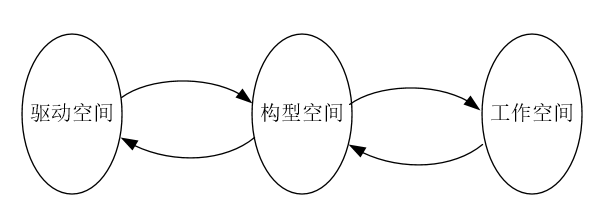
\includegraphics[height=4cm]{figures/map.png}
		\caption{连续型机器人的运动学组成}
		\label{fig:map}
	\end{figure}

	在研究这三类空间的映射关系时,一般先建立单个关节或单个臂段的运动学模型,然后利用链式法则推广成为整个机械臂的运动学模型。
	
	单个关节或臂段的驱动空间与构型空间之间的关系一般由几何关系建立。如图\ref{fig:single_joint}所示,位于单个关节之间的绳索长度可以等效成连接过孔的矢量长度$| \overrightarrow{B_i P_i}| $。由于圆盘上的过孔在各自的圆盘坐标系下的位置固定,因此在建立了两个圆盘坐标系($\{O x_{j-1} y_{j-1} z_{j-1}\}$ 和 $\{O x_{j} y_{j} z_{j}\}$)的坐标变换关系之后,即可得到绳索长度。
	\begin{figure}[h]
		\centering
		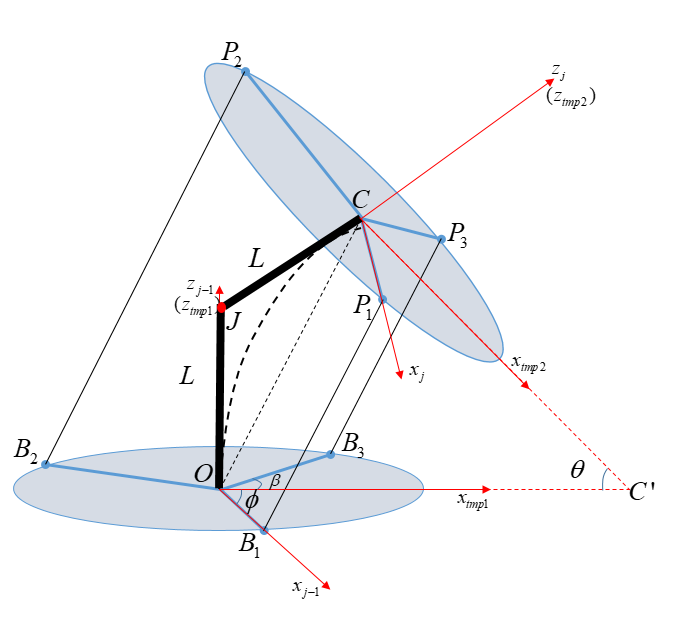
\includegraphics[height=7cm]{figures/single_joint.png}
		\caption{单个关节弯曲示意简图}
		\label{fig:single_joint}
	\end{figure}

	令$T_{j-1}^{j}$代表两个圆盘坐标系$\{O x_{j-1} y_{j-1} z_{j-1}\}$ 和 $\{O x_{j} y_{j} z_{j}\}$之间的齐次坐标变换,则绳索长度可以按照式\ref{eq:len}求解
	\begin{equation}
	| \overrightarrow{B_i P_i} | = \mathsf{C}_{\overrightarrow{OB_i}} - T_{j-1}^{j} \mathsf{C}_{\overrightarrow{C P_i}}  ||
	\label{eq:len}
	\end{equation}
	其中,$\mathsf{C}_{\cdot} $是$\cdot$在本体坐标系下的齐次坐标表示。
	
	虽然单个关节的驱动空间和构型空间之间的关系比较简单,但对于多个关节或臂段串联的机器人整体来说,这一映射关系可能会因为节间的耦合关系而变得复杂。远端臂段的驱动绳索往往要经由近端臂段过孔导引,因此近端臂段的弯曲变形会直接造成远端驱动绳索的长度变化,在计算远端的驱动参数时,应该补偿掉由于节间耦合带来的长度变化。
	
	构型空间与工作空间之间的关系由链式法则得到。对于具有$N$个关节或臂段的连续型机器人来说,其根部基座与末端位姿之间的齐次变换关系为:
	\begin{equation}
	T_{0}^{N} = \prod_{j=1}^{N} T_{j-1}^{j}
	\label{eq:chain}
	\end{equation}
	
	值得注意的是,在上述建立映射关系的过程中,所采用的都是几何上的关系,并未用到经典的D-H方法。因而在这种建模方法下,D-H方法的很多技巧和结论是很难直接运用的。受此影响,经典的Jacobian矩阵构造方法无法使用,需要另行推导简洁的雅可比矩阵构造方法。
	
	
	
	
\section{微分运动学模型的建立}
	得到机械臂的齐次变换之后,可以直接对变换矩阵进行求导并进行分离变量,以获得Jacobian矩阵\cite{hannan_kinematics_2003}。但这一非构造方法需要进行符号计算,并且计算量很大,限制了其应用。在建立运动学模型的过程中,我们采用的是几何关系,因此Jacobian矩阵应该也存在几何意义上的构造方法。
	
	对于图\ref{fig:single_joint}所示的由球铰连接的单个关节或臂段弯曲运动前后的齐次变换关系可以用旋量表示为:
	\begin{equation}
	T_{j-1, j} (\theta, \phi)= e^{\hat{\xi} \theta} T_{j-1, j}(\theta_0, \phi_0)
	\label{eq:ex_trans}
	\end{equation}
%	可以计算得到
%	\begin{equation}
%	e^{\hat{\xi} \theta} = T_{j-1, j} (\theta, \phi)T^{-1}_{j-1, j}(\theta_0, \phi_0)
%	\end{equation}
%	\begin{equation}
%	\omega = [-\sin\phi, \cos\phi, 0]^T
%	\label{eq:w}
%	\end{equation}
%	\begin{equation}
%	v = [-L\cos\phi, -L\sin\phi, 0]^T
%	\end{equation}
	进而可以得到空间速度如式\ref{eq:velocity}。
	\begin{equation}
	\begin{aligned}
	\hat{V}_{j-1,j}^{j-1} &= \dot{T}_{j-1,j}(\theta,\phi) {T}^{-1}_{j-1,j}(\theta,\phi)\\
	&=\frac{d}{dt}(e^{\hat{\xi} \theta}) T^{-1}_{j-1,j}(0,0) (T^{-1}_{j-1,j}(0,0))^{-1} (e^{\hat{\xi} \theta})^{-1}\\
	&=\frac{d}{dt}(e^{\hat{\xi} \theta})(e^{\hat{\xi} \theta})^{-1}
	\end{aligned}
	\label{eq:velocity}
	\end{equation}
	由于$\hat{\xi}$随弯曲方向变化,式\ref{eq:velocity}的简化需要借助于Lie Bracket工具。
	\begin{equation}
	\frac{d}{dt}(e^{\hat{\xi} \theta}) = dexp_{(\hat{\xi}\theta)} \frac{d(\hat{\xi}\theta)}{dt} e^{\hat{\xi} \theta}
	\label{eq:dexp}
	\end{equation}
	\begin{equation}
	dexp_{(\hat{\xi}\theta)} \frac{d(\hat{\xi}\theta)}{dt} = C + \frac{1}{2!}[A, C] + \frac{1}{3!}[A, [A, C]] + \cdots
	\label{eq:liebracket}
	\end{equation}
	其中,
	$$ [A, C] = AC-CA $$
	$$ A= \hat{\xi}\theta = \begin{bmatrix}
	\hat{\omega} & v \\
	\mathbf{0} & 0
	\end{bmatrix} \theta $$
	$$ C = \frac{d(\hat{\xi}\theta)}{dt}$$
	
	在得到单个关节的雅可比矩阵之后,则可以通过链式法则得到整个连续型机械臂的微分运动模型。
	

\section{运动学逆解及规划方法研究}
连续型柔性臂的逆解问题即是在给定期望位置后,计算每个关节臂段的弯曲角度和弯曲方向,进而利用构型空间与驱动空间之间的映射关系,得到绳索长度的变化。由于连续型柔性臂的高冗余度特点,位置级逆运动学求解难以解析获得,需要采取数值迭代等方法来解决。
\subsection{基于微分运动学的逆运动学求解}
基于微分运动学的逆运动学求解是借助于雅可比矩阵伪逆,在已知当前迭代位置$ \mathbf{p}_c $的情况下,利用位置误差$ d\mathbf{p} = \mathbf{p}_d -\mathbf{p}_c $得到构型参数的变化量$d\mathbf{q}$。经过不断的数值迭代,最终使得迭代位置于期望位置重合\cite{webster_closed-form_2009}。算法的流程图如\ref{fig:flowchart}所示。
\begin{figure}[!htpb]
	\centering
	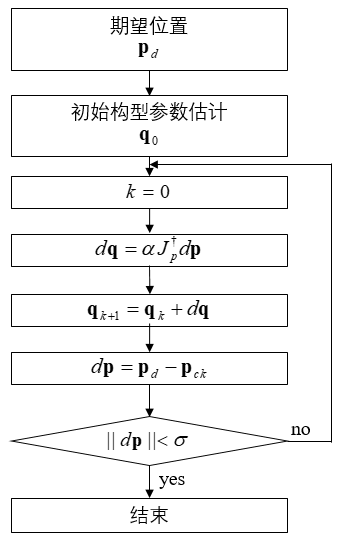
\includegraphics[width=5cm]{figures/flowchart.png}
	\caption{基于微分运动学的逆运动学求解流程图 }
	\label{fig:flowchart}
\end{figure}
\subsection{基于模态函数的逆运动学求解}
基于模态函数的逆解方法是由Chirikjian最早提出的\cite{chirikjian_obstacle_1990, chirikjian_geometric_1992}。被广泛应用于超冗余机械臂的逆运动学求解。这类方法的核心思想是用脊线刻画超冗余机械臂的宏观几何形状,进而将实际机械臂向这条脊线拟合,从而直接确定每一段关节所需的构型参数。脊线是分段连续的曲线,可以由给定的期望位置和模态函数经过迭代计算获得。采用这类方法进行连续型机械臂逆运动学求解的流程如图所示。
\begin{figure}[!htpb]
	\centering
	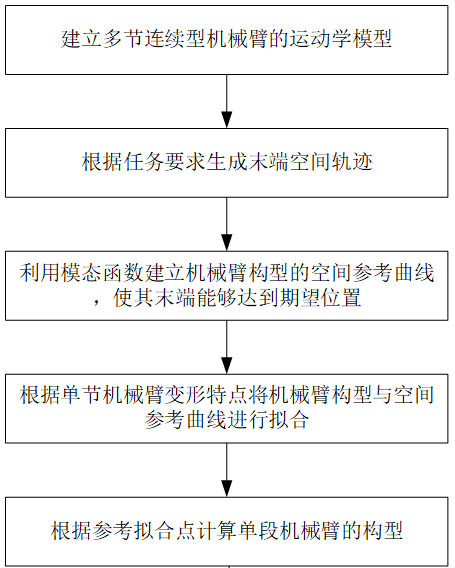
\includegraphics[width=6cm]{figures/flowchart_modal.png}
	\caption{基于模态函数的逆运动学求解流程图 }
	\label{fig:flowchart_modal}
\end{figure}